
\setchapterimage[6cm]{cabecera3}
\setchapterpreamble[u]{\margintoc}
%%%%%%%%%%%%%%%%%%%%%%%%%%%%%%%%%%%%%%%%%%%%%%%%%%%%%%%%%%%%%

\chapter{Arquitectura orientada a Servicios}
\label{ch:SOA}
\index{SOA}

La arquitectura del software es la estructura(s) del sistema que incluye componentes de software, las propiedades visibles externamente de esos componentes, las relaciones entre ellos y las restricciones sobre su uso.  Es una abstracción de los elementos de tiempo de ejecución de un sistema de software durante alguna fase de su operación. Un sistema puede estar compuesto por varios niveles de abstracción y fases de operación, cada una con su propia arquitectura de software. \cite{Fielding2000}.  


\section{Informática orientada a Servicios}
\index{informática orientada a servicios}

Informática orientada a Servicios representa una plataforma informática distribuida de nueva generación. 
 Incluye su propio \gls{paradigma de diseno} y principios de diseño,  \gls{patron de diseno}, lenguajes de patrones, un modelo arquitectónico distintivo y conceptos, tecnologías y marcos relacionados.
 \cite{Erl2007a}, \cite{Erl2008}
 
 \subsection{Elementos de Informática orientada a  Servicios}
 \index{ elementos de informática orientada a servicios}
 
 La \gls{informatica orientada a servicios} (Service-oriented computing, SOC) es un paradigma informático que utiliza los servicios como
 elementos para apoyar el desarrollo rápido y de bajo costo de aplicaciones/soluciones  distribuidas. La promesa de la informática orientada a servicios es un mundo de servicios cooperativos  que se acoplan libremente para crear  procesos comerciales dinámicos y aplicaciones ágiles  que puede abarcar organizaciones y plataformas informáticas, y que puede adaptarse de forma rápida y autónoma  a   requisitos cambiantes. (\sidecite{Buyya2013}, \sidecite{DimitriosGeorgakopoulos2009}, \sidecite{Erl2007}, \sidecite{Papazoglou2003} )
 
 Para construir el modelo de servicio, informática orientada a servicios se basa en la arquitectura orientada a servicios (SOA), que es una forma de reorganizar las aplicaciones de software y la infraestructura en un conjunto de servicios que interactúan.  A continuaci\'on, se presenta los elementos relacionados con el parad\'igma de la inform\'atica orientada a servicios: SOA, servicios, orquestación de servicios,   coordinación de transacciones de servicios,  y otras cuestiones que se aplican a los componentes de una arquitectura orientada a servicios.
 
  
 
\paragraph{Arquitectura orientada a Servicios}
 \index{ SOA}

Arquitectura orientada a Servicios establece un modelo arquitectónico orientado a mejorar la eficiencia, la agilidad y la productividad de una empresa mediante el uso de la informática orientada a servicios.
 La plataforma informática orientada a servicios gira en torno al paradigma de diseño de orientación de servicio y su relación con SOA. 
 Una implementación de SOA puede consistir en una combinación de tecnologías, productos, API, extensiones de infraestructura de soporte y otros elementos.
 
 
 \paragraph{Servicios y orientación a servicios}
 \index{ servicios}
 \index{ orientación a servicios}
 
La  \gls{orientacion a servicios} es un paradigma de diseño compuesto por un 	conjunto específico de principios de diseño.   La aplicación de estos principios al diseño de solución lógica da como resultado una solución orientada al servicio.
 La orientación a servicio usa la separación de problemas y da forma a la solución. 	Aplicar la orientación a servicios  da como resultado una solución que se puede clasificar de forma segura como \textbf{orientada a servicios} y unidades que se califican como \textbf{servicios}. 
 
  El \textbf{\gls{servicio}} es la unidad fundamental de la solución orientada a servicios.  Cada servicio tiene su propio contexto funcional y capacidades relacionadas con este contexto.  En la figura \ref{fig:servicio} esta ilustrado la notaci\'on usada para modelar un servicio (izquierda) y de describir un  servicio con sus capacidades (derecha).
  
  En  \sidecite{W3C2022}, un servicio es recurso abstracto que representa una capacidad de realizar tareas que constituyen una funcionalidad coherente desde el punto de vista de los proveedores de las entidades y de las entidades solicitantes.  

  
   			 
 	\begin{figure}%
 %	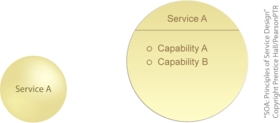
\includegraphics{7/servicio.png}
 	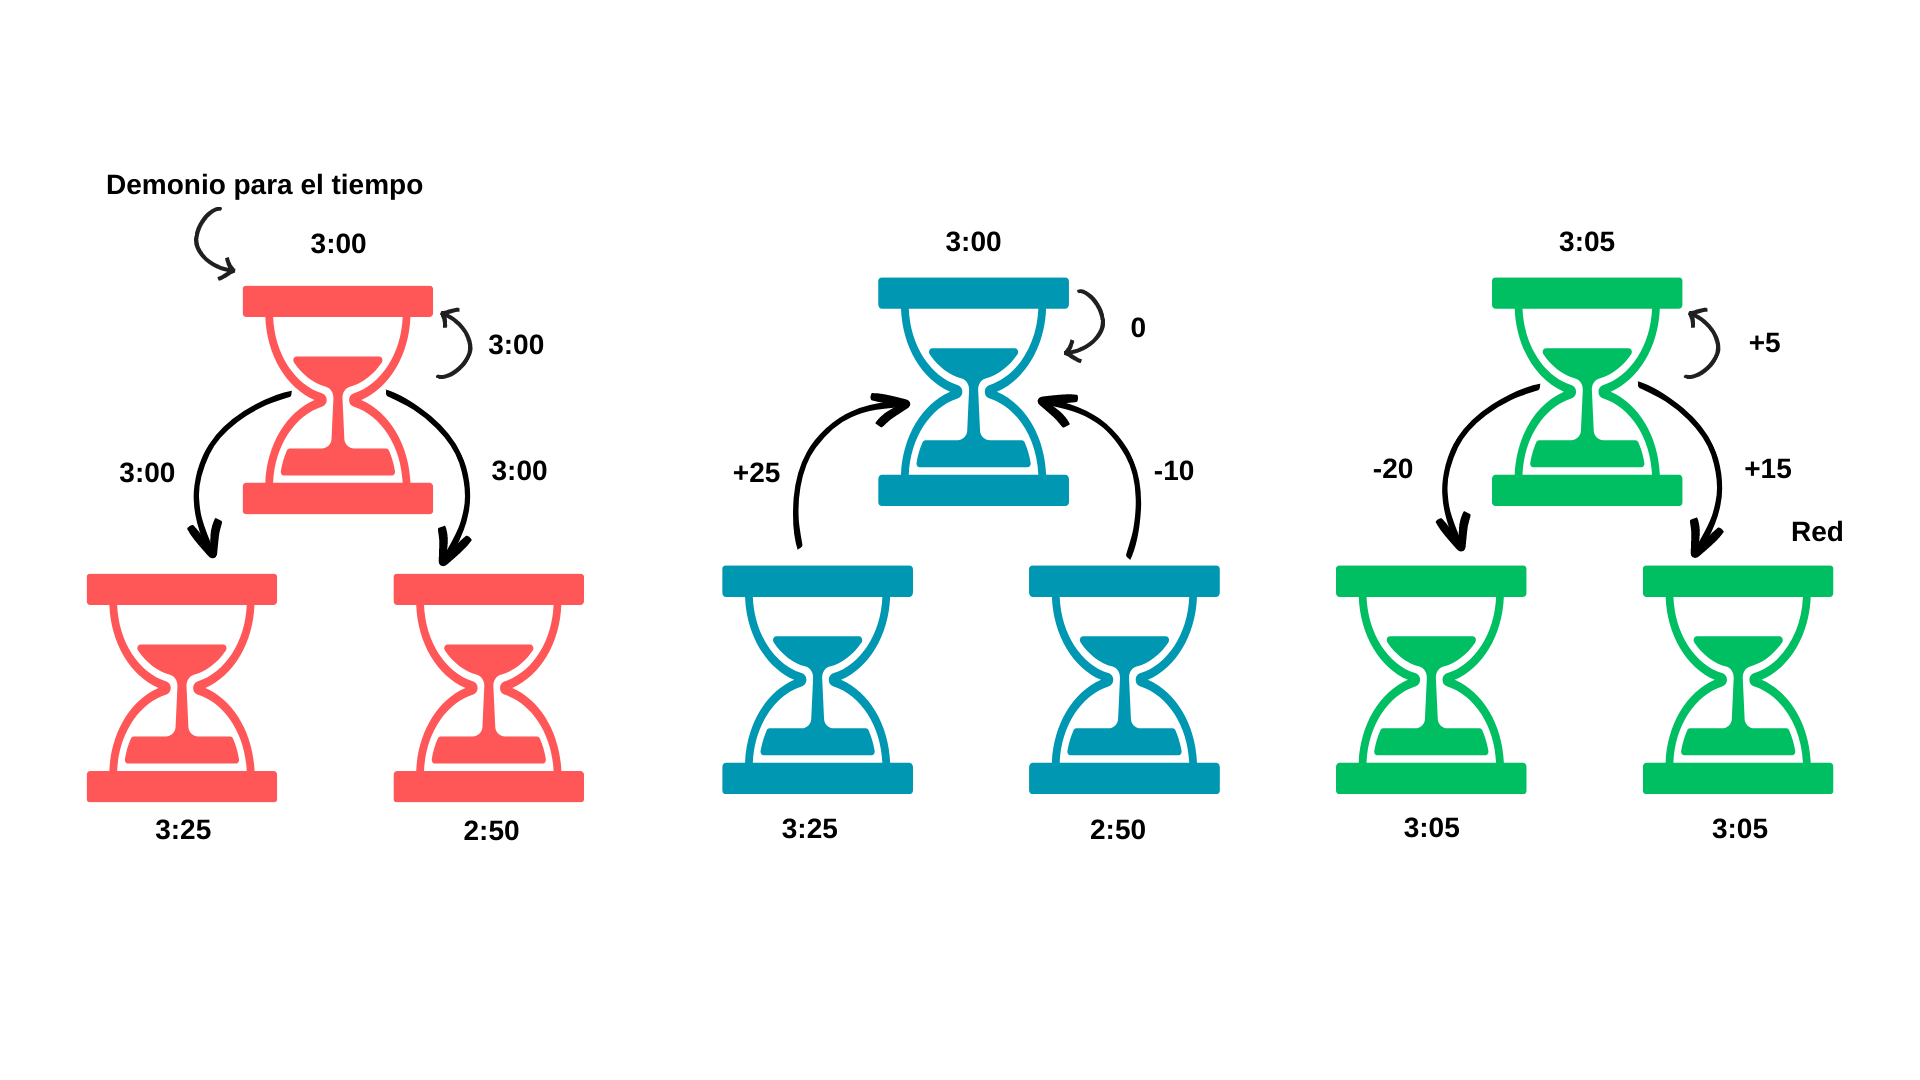
\includegraphics{7/1.png}
 	\caption{Servicios y sus capacidades}
 	\label{fig:servicio}
 \end{figure}
 
 Aquellas capacidades adecuadas para la invocación de programas de consumo externos se expresan a través de un \textbf{contrato de servicio} publicado. Un contrato de servicio establece las cualidades que son (o deberían ser) visibles para los negocios entre los participantes del servicio, en lugar de   modelar interacciones en un  nivel detallado. Las partes de un contrato de servicios se ilustran en la figura \ref{fig:contrato}. 
 
 \begin{figure}%  	
 %	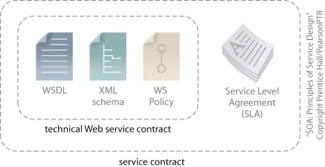
\includegraphics{7/contrato.png}  
 		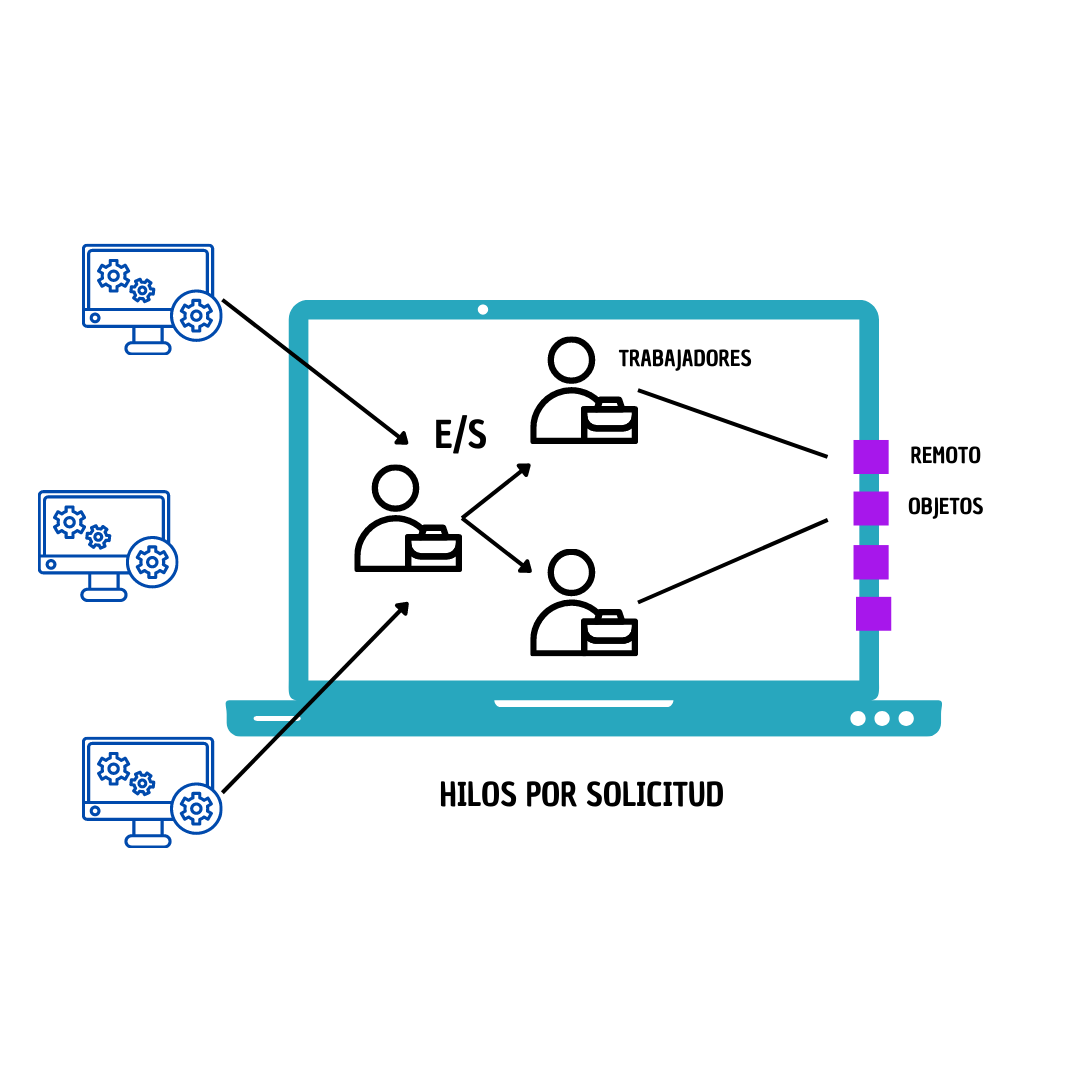
\includegraphics{7/2.png} 
 		\caption{Contrato de Servicios.}  
 		\label{fig:contrato}  
 \end{figure}
 
 \paragraph{Composición de Servicios}
  \index{ composición de servicios}
 
  Una \gls{composicion de servicios} es un agregado coordinado de servicios. Es comparable a una aplicación tradicional, ya que su alcance funcional suele asociarse con la automatización de un proceso empresarial principal.  
  Un ejemplo de modelado de composiciones de servicios esta en la figura \ref{fig:composicion}. Es una composición de servicio compuesta por cuatro servicios. Las flechas indican una secuencia de modelados de  intercambios de  mensajes. La flecha 5 representa una entrega de datos asíncrona unidireccional del Servicio A al Servicio D.
  
  	\begin{figure}%
  	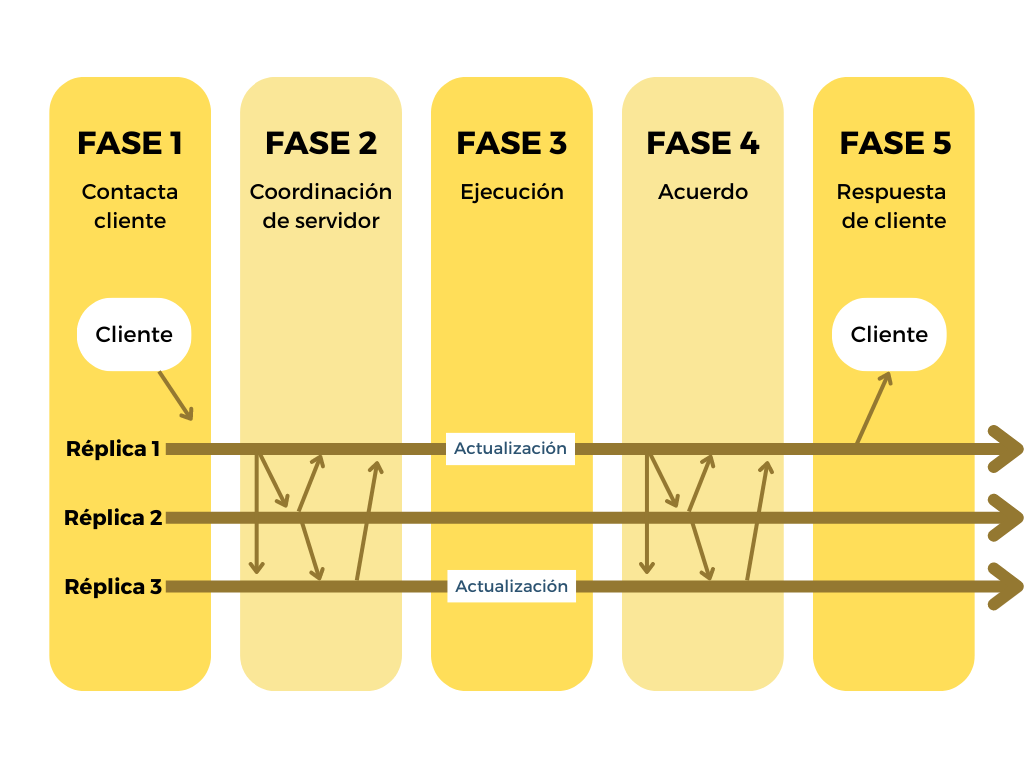
\includegraphics{7/3.png}
  	\caption{Composición de Servicios. Adaptado de \ER}
  	\label{fig:composicion}
  \end{figure}
  
  
  \paragraph{Inventario de Servicios}
 \index{inventario de servicios}
  
 
 un \gls{inventario de servicios} es una colección de servicios que representa una empresa o un segmento de ella, ver figura \ref{fig:inventario}. Son creados a través de procesos top-down que resultan en la definición del inventario de servicio. Los principios de diseño y los estándares de diseño aplicados al inventario  establece el grado de interoperabilidad interservicios. 
  
  
  \begin{figure}%
  	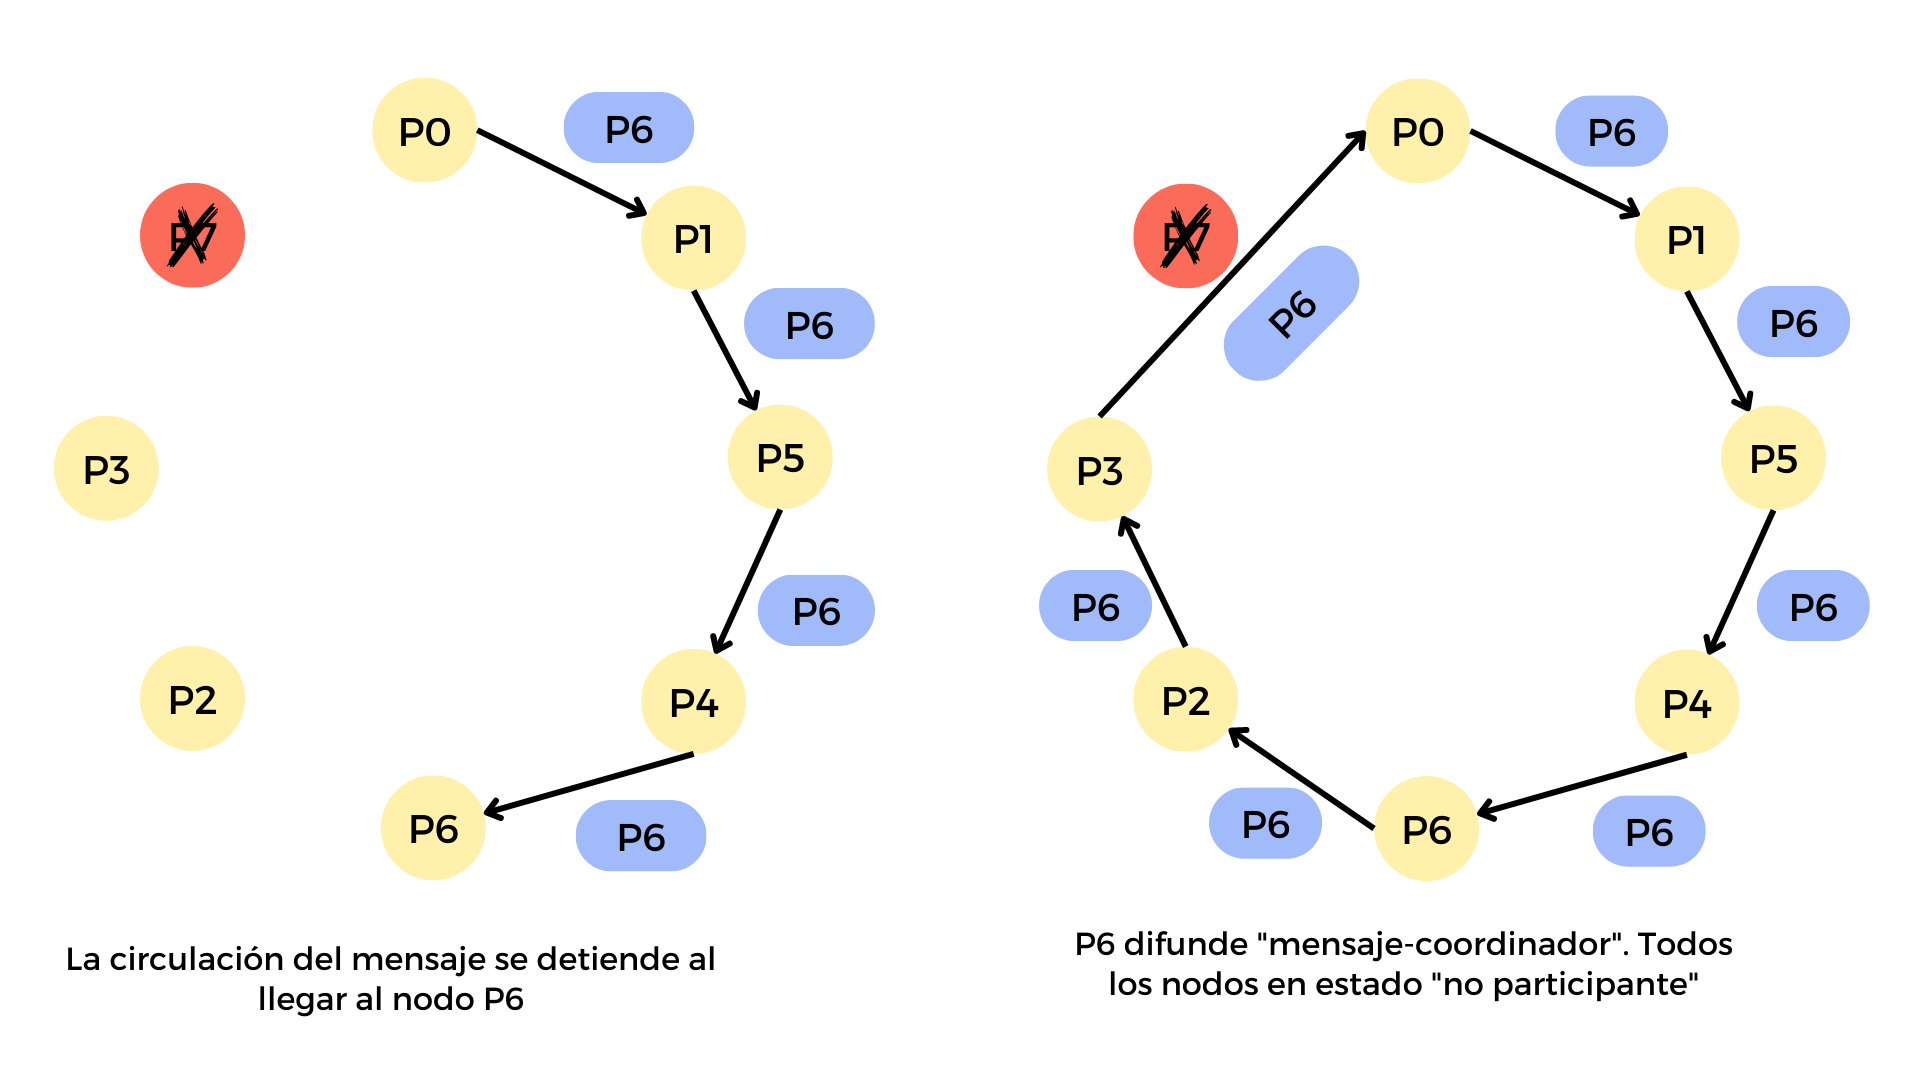
\includegraphics{7/4.png}
  	\caption{Inventario de Servicios}
  	\label{fig:inventario}
  \end{figure}
  
 % \paragraph{Vista Conceptual de Servicios}     \index{informática orientada a servicios!vista conceptual}
  
%%  \begin{itemize}    	\item SOA es resultado del diseño de la arquitectura tecnológica en apoyo a la solución orientada a servicios, conformada por servicios y servicios compuestos configurados y diseñados de acuerdo con la orientación del servicio.    	\item  La orientación al servicio es un paradigma de diseño compuesto por principios de diseño orientados a servicio.     	\item Cuando se aplican a unidades de solución lógica, estos principios crean servicios con características de diseño que respaldan los objetivos generales y la visión de la informática orientada a servicios.      	\item La informática orientada al servicio es una plataforma informática  que abarca el paradigma de orientación al servicio y SOA con el objetivo de crear y ensamblar uno o más inventarios de servicios.     \end{itemize}     \begin{figure}%    	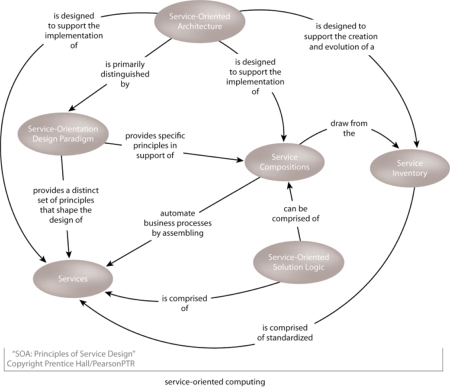
\includegraphics{7/VistaConceptual.png}    	\caption{Vista Conceptual  de Servicios}    	\label{fig:vista-concep}   \end{figure}
  
 \paragraph{Vista F\'isica  de Servicios}
     \index{ vista f\'isica de servicios}
  
   La solución orientada al servicio se implementa como servicios y servicio compuestos diseñadas de acuerdo con principios de diseño de orientación de servicio, figura \ref{fig:vista-fisic}.
   Un servicio puede ser invocado por múltiples programas de consumidores. 
  	Los servicios compuestos puede formar la base de un inventario de servicios que se administran independientemente de su propio entorno de despliegue físico.
	Se pueden automatizar múltiples procesos comerciales mediante los servicios compuestos.
   	Debido a que los servicios son reutilizables, no pertenecen a ningúna aplicación.
 
    \begin{figure}%
  	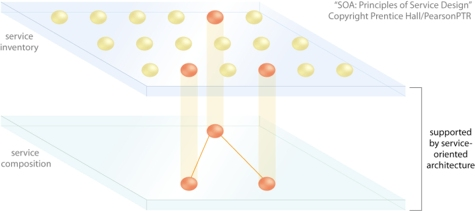
\includegraphics{7/VistaFisica.png}
  	\caption{Vista F\'isica  de Servicios. Tomado de \ER}
  	\label{fig:vista-fisic}
  \end{figure}
  
   
    \subsection{Principios de diseño de orientación de servicio}
   % -------------------------------------------------
   \paragraph{Contrato de servicio estandarizado}
      \index{contrato de servicios}
   	 
   	
   	Los servicios expresan su propósito y capacidades en un contrato de servicio.  El principio de diseño del contrato requiere  consideraciones de diseño de la interfaz del servicio.
   	Diseño incluye la manera en que los servicios expresan la funcionalidad, definición de tipos y modelos de datos, las políticas, etc.  

   		
   	%%	 \begin{figure}%     			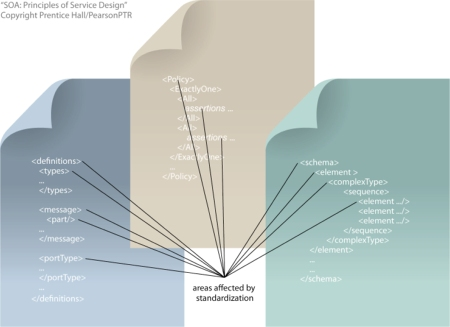
\includegraphics{7/dis-contrato.png}      			\caption{Contrato de Servicios}   	\label{fig:contrato2}      		\end{figure}
   		

 \paragraph{Acoplamiento }
    \index{acoplamiento}
   
 	El \gls{acoplamiento} es una conexión o relación entre dos cosas. Comparable a un nivel de dependencia. 
 	La orientaci\'on al servicio aboga por la creación de un tipo específico de relación dentro y fuera de los límites del servicio, que reduzca las dependencias entre el contrato, implementación y consumidores del servicio .
 	Acoplamiento débil o \gls{debilmente acoplado} promueve el diseño independiente, evolución e implementación de un servicio, al tiempo que garantiza la interoperabilidad con los consumidores del servicio.   
 	
 	\paragraph{Abstracción}
 	   \index{abstracción}
 	  
 	 Este principio enfatiza la necesidad de ocultar la mayor cantidad de detalles subyacentes de un servicio como sea posible. 
 	Es importante para habilitar y preserva la relación débilmente acoplada y, también en el posicionamiento y diseño de composiciones de servicio.
 	 Los metadatos son relevantes cuando se evalúan los niveles de abstracción apropiados.   
 	
 		
 	\paragraph{Reutilización de servicio}
 	 \index{reutilización de servicios}
 	  La reutilización se enfatiza fuertemente dentro de la orientación del servicio; es una parte central de los  procesos de análisis y diseño de servicios, y también forma la base para los modelos claves de servicio.
 	 El principio de la reutilización del servicio enfatiza el posicionamiento de los servicios como recursos empresariales con contextos funcionales agnósticos.   
 	 
 	 
 	 \paragraph{Autonomía del servicio}
 	   \index{ autonomía de servicios}
 	  
 	  La autonomía es necesaria para que los servicios puedan llevar a cabo sus capacidades de manera consistente y confiable
 	 Es necesaria la aplicación de principios de diseño para aumentar la confiabilidad y predictibilidad del comportamiento de un servicio.   
 	 Se considera niveles de aislamiento y consideraciones de normalización del servicio para lograr una medida adecuada de autonomía.  
 	  
 	 	
 	 \paragraph{Servicio sin estado}
 	  	   \index{ servicio sin estado}
 	  	 
 	 	El manejo de información con estado  puede comprometer la disponibilidad y escalabilidad de un servicio. Los servicios se diseñan para permanecer con estado solo cuando sea necesario. 
 	 	El principio de servicios \gls{sin estado} requiere que se evalúen la idoneidad de la arquitectura tecnológica para proporcionar las opciones de delegación y diferimiento de la administración de los estados.  
 	  
 	 \paragraph{Descubrimiento de servicio}
 	  \index{descubrimiento de servicio}
  
 	  Para que los servicios se posicionen como activos, deben identificarse y comprenderse cuando se presenten oportunidades de reutilización.El diseño del servicio debe tener en cuenta la \textit{\textit{calidad de las comunicaciones}} del servicio y sus capacidades individuales. 
 	  
 
 %%%%%%%%%%%%%%%%%%%%%%%%%%%%%%%%%%%%%%%%%%%%%%%%%%%%%%%%%%%%%%%%%%%%%%%%%%%%%%%%%%%%%%%%%%%%%%%%%%%%%%%%%%%%%%%%%%%%%%%%%%%%%%%%%%%%%%%%%%%%%%%%% 
 
  \section{Servicios Web}
   \index{servicios web}
   
   De acuerdo a \sidecite{W3C2022}, un \gls{servicio web} es un sistema software diseñado para soportar la interacción máquina-a-máquina, a través de una red, de forma interoperable. Cuenta con una interfaz descrita en un formato procesable por un equipo informático (específicamente en \textbf{WSDL}), a través de la que es posible interactuar con el mismo mediante el intercambio de mensajes \textbf{SOAP}, típicamente transmitidos usando serialización XML sobre HTTP conjuntamente con otros estándares web.
   
   La Figura \ref{fig:infraestructura} indica los puntos principales sobre la arquitectura de comunicación en la que operan los servicios web: un servicio web se identifica mediante un URI y los clientes pueden acceder a él mediante mensajes formateados en XML \sidecite{Coulouris2011}.    
   SOAP se utiliza para encapsular estos mensajes y transmitirlos a través de HTTP u otro protocolo, por ejemplo, TCP o SMTP. Un servicio web implementa descripciones de servicios para especificar la interfaz y otros aspectos del servicio en beneficio de los clientes potenciales.
    	
 \begin{figure}%
 	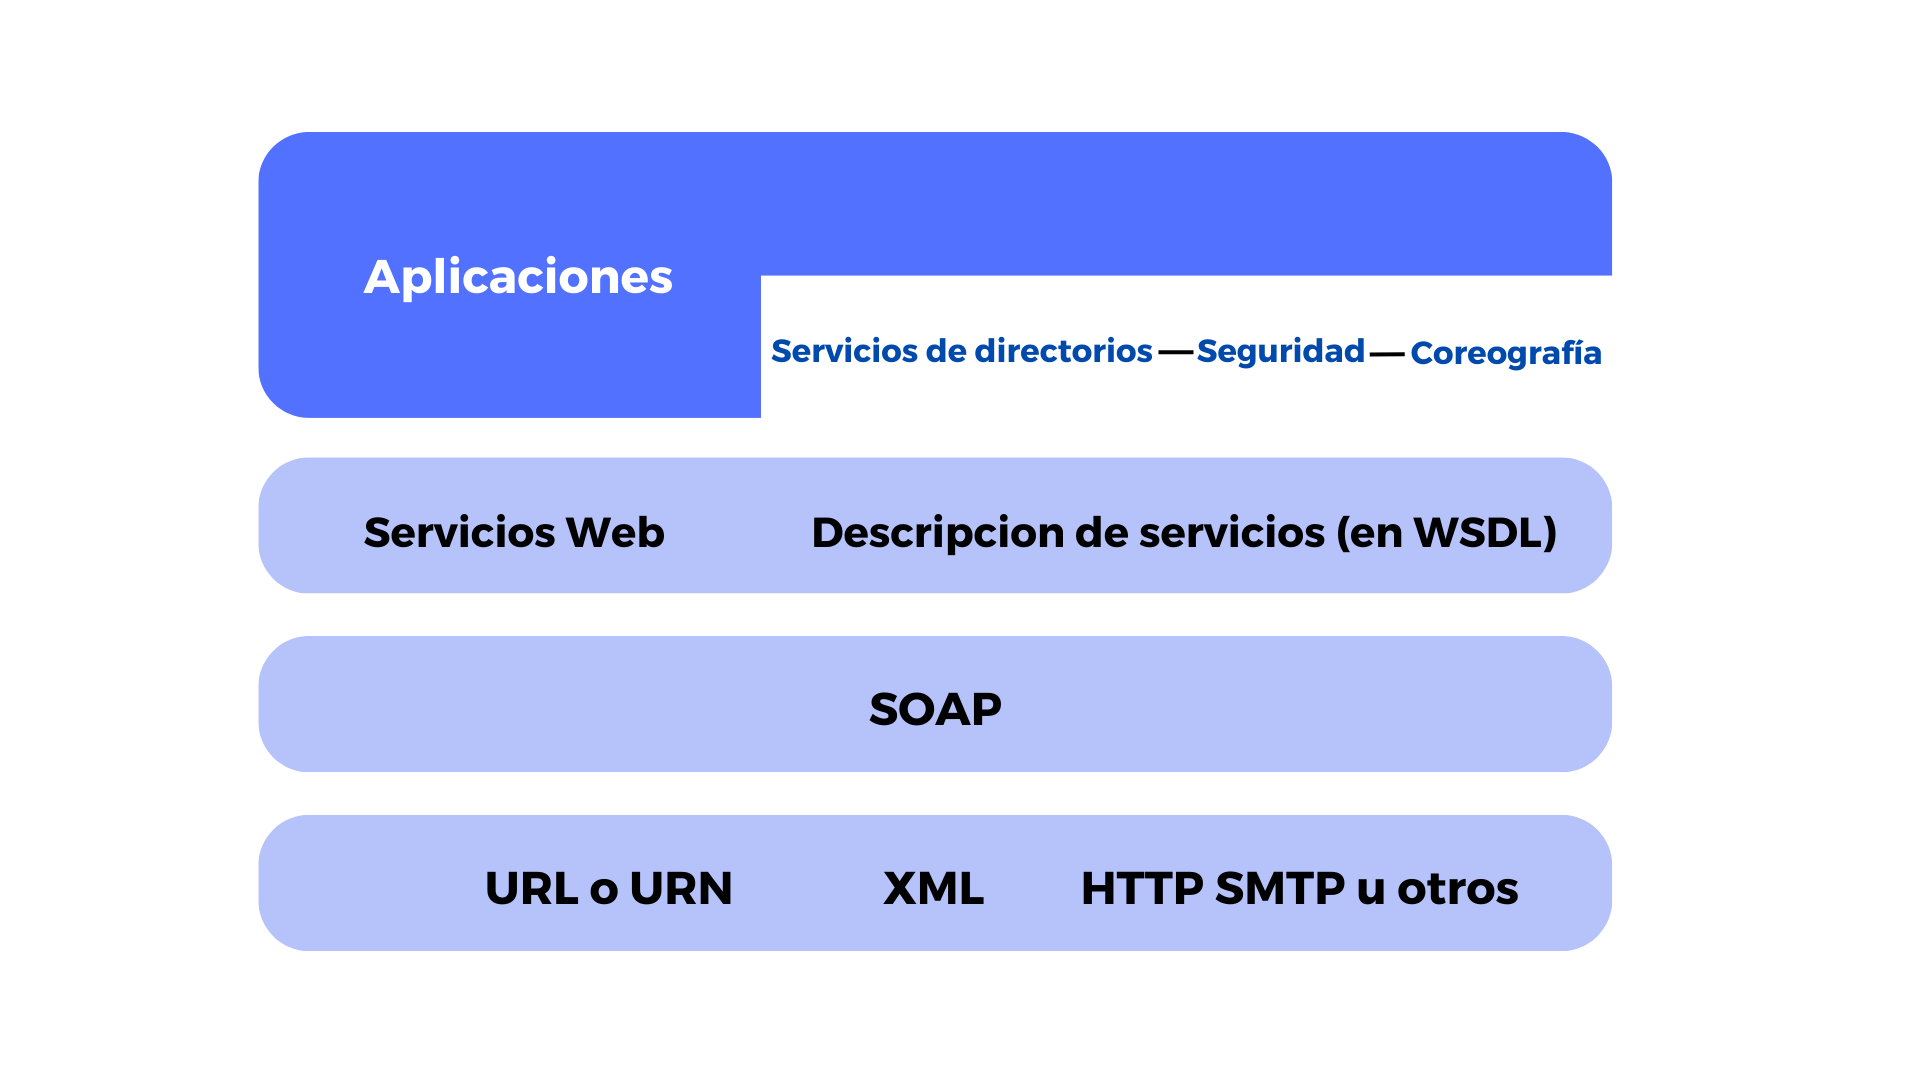
\includegraphics{7/6.png}
 	\caption{Infraestructura de Servicios Web.}
 	\label{fig:infraestructura}
 \end{figure}
 
Las características distintivas de los servicios web se listan a continuaci\'on:
 		\begin{itemize}
 			\item Uso de SOAP 
 			\item Uso de XML: la representación del mensaje en  XML para protocolos de comunicaci\'on y datos.   El formato XML es fácil de leer y entender, lo que facilita la creación y el mantenimiento de archivos XML. Su desventaja es el espacio que ocupa la representación textual y el tiempo de procesamiento (parse).   
 			\item Combinación con otros servicios web para construir otras funcionalidades 
 			\item Patrones de comunicación: RR síncronos  RR asíncronos, combinaciones de ellos.  		   		
 	
 			\item Acoplamiento Débil: minimizar las dependencias entre servicios para tener una arquitectura flexible 			
 			\item Uso de \gls{interfaz de servicio web} 		
 			\item Tendencia a la simplicidad: ejm, REST usa interfaces mínimas (GOOGLE) 			
 			\item	Uso de múltiples paradigmas de comunicación (RR, Asíncronos, indirectos). Esto afecta el nivel de acoplamiento.    		
 	 	\end{itemize}
 		
 	
 	  \subsection{SOAP}
 	        \index{SOAP}
 	  
 	   SOAP (SOAP, Service Oriented Architecture Protocol) es un protocolo estándar que define cómo dos objetos en diferentes procesos pueden comunicarse por medio de intercambio de datos XML \sidecite{W3C2022}.
 	    		
 	  Su propósito es establecer una interacción asíncrona entre el cliente y el servidor.  Define un esquema con XML, donde se representa el contenido de una solicitud – respuesta de un mensaje
 	  Se usa con protocolos HTTP, SMTP, TCP, UDP.
 	  La estructura de un mensaje SOAP se muestra en el listado \ref{list:soap-est}:
 	  
  
 	  \begin{lstlisting}[label=list:soap-est,caption=Estructura de mensaje SOAP]
 	 	<soap:Envelope>
 		 	<soap:Header>
 	 			<header element>
				</header element>
 	 		</soap:Header>
 	 		<soap:Body>
 	 			<body element>
 	 			</body element>
  	 		</soap:Body>
 	 	</soap:Envelope>
 	 \end{lstlisting} 
 	 
 	
 
 	  	 
 	 Un mensaje SOAP puede ser un documento o un soporte a la comunicación cliente-servidor:
 	\begin{itemize}
 		\item	Un documento  se coloca directamente en el interior del elemento de cuerpo  junto con una referencia a un esquema XML que contiene la descripción del servicio (nombres y tipos utilizados en el documento). 
 		\item Para la comunicación cliente-servidor, el elemento del cuerpo \textit{body} contiene ya sea una solicitud (\textit{Request}), ver listado \ref{list:soap-sol}  o una respuesta (\textit{Replay}), ejemplo en el listado \ref{list:soap-resp}.
 	\end{itemize}
 
 
 
   \begin{lstlisting}[label=list:soap-sol, caption=Solicitud en mensaje SOAP. Tomado de \WC]  <soap:Envelope xmlns:soap="http://schemas.xmlsoap.org/soap/envelope/">
  	<soap:Body>
 		 <getProductDetails xmlns="http://warehouse.example.com/ws">
 			 <productId>827635</productId>
  		</getProductDetails>
	</soap:Body>
  </soap:Envelope>
 \end{lstlisting}
 
 
 
 
 \begin{lstlisting} [label=list:soap-resp, caption=Respuesta en mensaje SOAP. Tomado de \WC]
   <soap:Envelope xmlns:soap="http://schemas.xmlsoap.org/soap/envelope/">
 		<soap:Body>
 			<getProductDetailsResponse xmlns="http://warehouse.example.com/ws">
 				<getProductDetailsResult>
 					<productName>Toptimate 3-Piece Set</productName>
					<productId>827635</productId>
 					<description>3-Piece luggage set.  Black Polyester.</description>
					<price>96.50</price>
 					<inStock>true</inStock>
 				</getProductDetailsResult>
 			</getProductDetailsResponse>
 		</soap:Body>
 </soap:Envelope>
\end{lstlisting}


 
 
   	\paragraph{SOAP: Protocolo de Transporte del mensaje} 
   	Se requiere un protocolo de transporte para enviar un mensaje SOAP
   	 a su destino. Los mensajes SOAP son independientes del tipo de transporte utilizado. HTTP  se usa para especificar la dirección de destino del mensaje. De igual manera,   se usa  HTTP  para retornar el contenido de un respuesta a una solicitud SOAP. En el listado \ref{list:soap-http}: las l\'ineas de la 1 a la 4 es el encabezado de HTTP, a partir de la 4 se detalla el mensaje SOAP. 
 
 
 
 	\begin{lstlisting}[label=list:soap-http, caption=Protocolo de Transporte en SOAP. Tomado de \CO]
 		POST /examples/stringer
 		Host: www.cdk4.net
 		Content-Type: application/soap+xml
 		Action: http://www.cdk4.net/examples/stringer#exchange
 		
 		<env:envelope xmlns:env = namespace URI for SOAP envelope>
 			<env:header> </env:header>
 				<env:body> </env:body>
 		</env:Envelope>
 	\end{lstlisting}
 	
 	
 En cuanto a la confiabilidad en la comunicaci\'on del mensaje usando SOAP, debido a que SOA  usa  HTTP sobre TCP por lo que esta afectado por el modelo de fallas de TCP ya descrito en cap\'itulo \ref{ch:Potocolos capa de Transporte}	
 
 \paragraph{B\'usqueda de un servicio en la web}
 
 En la figura \ref{fig:soap-http} se muestra c\'omo es la b\'usqueda de un servicio en la web y los actores involucrados en ello:
 
 \begin{enumerate}
 	\item ?` Donde consigo un servicio X? la pregunta se hace al directorio de servicios, el \textbf{UDDI}    
 	\item El \textbf{UDDI} responde: el Servidor A es capaz de hacer X. 
 	\item ?` C\'omo invoco su servicio?                       
 	\item Mire el \textbf{WSDL}  que esta disponible    
 	\item Hago la solicitud X usando el protocolo SOAP                  
 	\item Hago la solicitiud de la  operacion X usando el protocolo \textbf{SOAP}
 \end{enumerate}
   
   
   	 \begin{figure}%
   		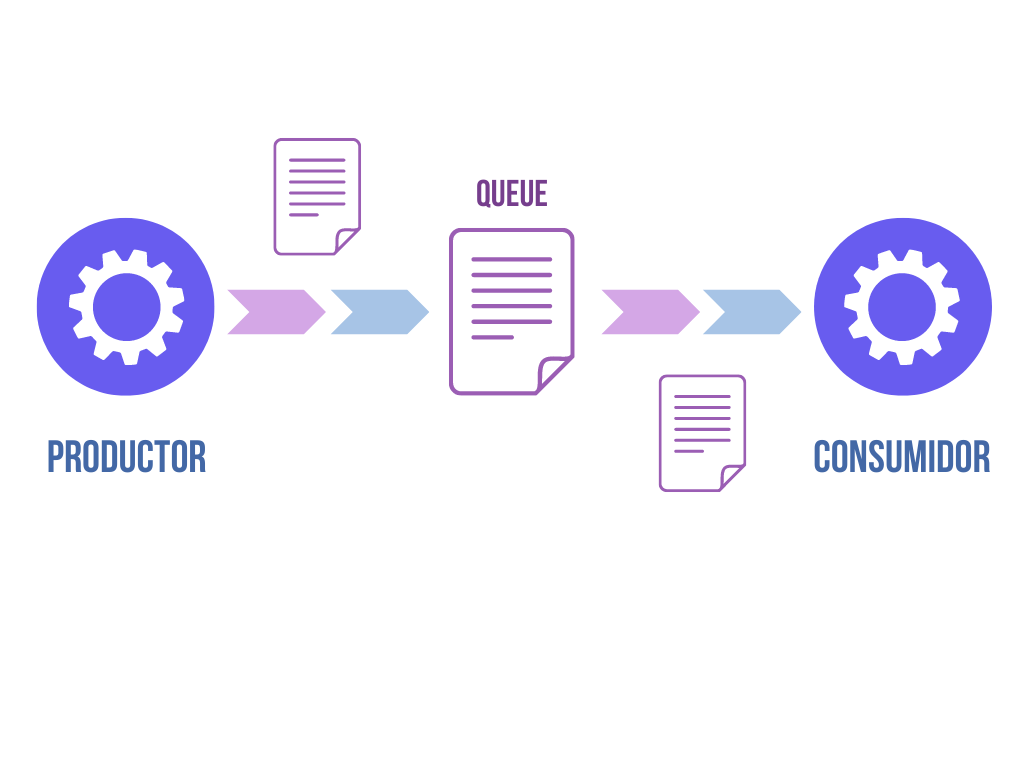
\includegraphics {7/7.png} 
   		\caption{Servicio Web con SOAP y HTTP}
   		\label{fig:soap-http}
   	\end{figure}
   	
   	
   
	\subsection{Descripci\'on de Servicios e Interfaces Web}
 La \gls{interfaz de servicio web} se hacen necesarias para permitir la comunicación de los clientes con los servicios.  La definición de las interfaces son proporcionadas por la descripción de servicios		 			
 
 La descripci\'on de Servicios  especifica como los mensajes son comunicados y la ubicaci\'on de ese servicio o el URI del servicio. 	
 Es un acuerdo entre cliente y servidor de como se ofrece un servicio. 	
 Se usa para generar procedimientos (stub) del cliente que  implementa el comportamiento  del cliente  			
 
 \subsection{Lenguaje de Descripci\'on del Servicio}
 	      \index{WSDL}
 
  El Lenguaje para Descripción de Servicios Web (WSDL, Web Service Description Language)  se usa para describir los servicios. WSLD define, usando esquema XML, la representación de los componentes de la descripción de servicios. 
 De igual manera, contempla la definición de nombre de elementos, tipos, mensajes, interfaz, enlaces y servicios. 			
 	 	 
 
 	Los elementos en la descripci\'on del servicio WSDL 
 			\begin{itemize} 
 				\item \textbf{Abstracta}: conjunto de definiciones de los tipos usados por el servicio
 				\begin{itemize} 
 					\item Tipo: <element name="isFilled" type="boolean"/>
 					\item Mensaje:descripción del mensaje que se intercambiará. También describe los tipos de mensajes
 				\end{itemize}
 				\item \textbf{Concreta}: enlace y servicio, ambas dependen del protocolo que se use en SOAP.
 			\end{itemize}
 
 \begin{figure}%
 	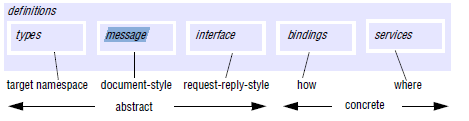
\includegraphics {7/service-idl} 
 	\caption{IDL}
 	\label{fig:wsdl-idl}
 \end{figure}
 
 \subsection{Descripci\'on  de los elementos de WSDL}
 
 \paragraph{Elemento \textit{Definitions}}

 Todas las partes de las descripciones abstractas y concretas se alojan dentro de un elemento raíz  que establece un constructo padre llamado \textit{Definitions}. Por lo tanto, lo que hay entre los elementos \textit{Definitions} representa el ámbito de un contrato de servicio Web  de un servicio Web, ver listado \ref{wsdl-element}.
 
 \begin{lstlisting}[label=wsdl-element, caption=Elemento \textit{Definitions}. Tomado de \WC]
 	<definitions name="OrdenCompra" targetNamespace= 		"http://example.com/contract/po" ...>
 				...
 	</definitions>
 \end{lstlisting}
 
 Este elemento tiene dos atributos opcionales: \textit{name} y \textit{target-Namespace}. Pueden añadirse  atributos adicionales como los atributos xmlns utilizados para establecer un rango de prefijos para los espacios de nombres existentes relevantes para este contrato. Estos prefijos se utilizan para identificar y distinguir elementos de distintos orígenes (con diferentes espacios de nombres) que residen en la misma definición WSDL.
 
 \begin{description}
 	\item[Atributo \textit{targetNamespace}]  El atributo \textit{targetNamespace}   establece el valor del espacio de nombres asociado a todos los elementos con nombre definidos en el documento \textbf{WSDL}.
 	Por ejemplo, el nombre de un elemento \textit{portType} definido en la definición WSDL está automáticamente
 	asociado con este espacio de nombres de destino, y por lo tanto será distinguible de nombres idénticos en diferentes definiciones WSDL.
 	
 	\item[Atributo \textit{xmlns}] Al igual que otro elemento XML, el elemento \textit{definitions} puede contener múltiples variaciones del atributo xmlns para establecer una serie de prefijos de espacio de nombres. Estos prefijos son necesarios cuando se necesita mezclar elementos de diferentes orígenes en el mismo documento.
 	Una definición WSDL básicamente siempre acabará conteniendo elementos de lenguajes distintos de WSDL (como \textbf{SOAP} y \textit{XML Schema}) y definiciones diferentes (como tipos definidos en otros documentos de esquema XML).  
 	
 	
 	\begin{lstlisting}[label=wsdl:attr-xmlns, caption= Atributo {xmlns}. Tomado de \ER]
 		<definitions name="OrdenCompra" targetNamespace=
 		"http://prueba.com/contract/po"
 			xmlns="http://schemas.xmlsoap.org/wsdl/"
 			xmlns:tns="http://prueba.com/contract/po"
 			xmlns:wsdl="http://schemas.xmlsoap.org/wsdl/"
 			xmlns:po="http://prueba.com/schema/po"
 			xmlns:soap11="http://schemas.xmlsoap.org/wsdl/soap/"
 			xmlns:soap12="http://schemas.xmlsoap.org/wsdl/soap12/">
 	\end{lstlisting}
 	
 	 Por ejemplo, los atributos \textit{xmlns} que pueden ser necesarios:
 	\begin{itemize}
 		\item  El atributo \textit{targetNamespace} se establece en \url{http://prueba.com/contract/po}, lo que significa que todos los elementos con nombre en la definición \textbf{WSDL} pertenecerán a este  espacio de nombres
 		\item  El espacio de nombres predeterminado se establece en el espacio de nombres \textbf{WSDL}, lo que indica que el espacio de los elementos estándar WSDL (tipos, portType, mensaje, etc.) no requerirán ningún prefijo  	cuando se utiliza en el documento, como se muestra a continuación:
 		
 	 
 		\begin{lstlisting}
 			<message name="msgOrdenCompraRequest">
 				<part name="OrdenCompra" element="po:ordenCompra"/>
 			</message>
 		\end{lstlisting}
 		
 		\item El prefijo \textit{tns}: está asociado con \url{http://prueba.com/contract/po}, que también es el espacio de nombres de destino. Esto permite referirse a elementos que pertenecen a la
 		espacio de nombres de destino en el documento WSDL a través de este prefijo.
 		
 		\item El prefijo \textit{po}: permite referirse a elementos del esquema XML que fueron declarados en el espacio de nombre   \url{http://prueba.com/schema/po},  como por ejemplo:
 		
 		\begin{lstlisting}
 			<message name="msgEnviarOrdenRequest">
 				<part name="OrdenCompra" element="po:ordenCompra"/>
 			</message>
 		\end{lstlisting}
 		
 		\item Los prefijos  \textit{soap11} y \textit{soap12} están vinculados al espacio de nombres estándar  para SOAP 1.1 y SOAP 1.2, respectivamente y se utilizan exclusivamente dentro de la  descripción \textbf{concreta} referida en la figura \ref{fig:wsdl-idl}.
 		
 	\end{itemize}
 	
 	\item[Elemento \textit{Documentation}]
 	Cualquier parte de una definición WSDL se puede anotar con comentarios legibles por humanos a través del uso del elemento de \textit{documentation}. Cualquier parte o elemento WSDL puede ser documentado, y su contenido puede ser texto arbitrario o incluso otros elementos XML.
 	
 	\begin{lstlisting}
 		<documentation>
 			Esta es una entidad de servicio responsable de los procesos de compra.
 		</documentation>
 	\end{lstlisting}
 		
 \end{description}
 
 \paragraph{Estructura del mensaje WSDL}
 
 
 En el nivel abstracto, un servicio web se define en términos de su interfaz pública. La descripci\'on  abstracta establece esta interfaz a través de un conjunto de elementos relacionados.
  La estructura de un mensaje WSDL se ve en el listado \ref{list:wsdl-est} 
 
 \begin{lstlisting}[label=list:wsdl-est, caption=Estructura de mensaje WSDL]
 	<definitions>
 		<types>
 			data type definitions........
 		</types>
 		<message>
 			definition of the data being communicated....
 		</message>
 		<portType>
 			set of operations......
 		</portType>
 		<binding>
 			protocol and data format specification....
 		</binding> 
 	</definitions> 
 \end{lstlisting}
 
 
 La estructura de la descripción abstracta (\sidecite{W3C2022} \sidecite{Erl2008}):
 \begin{description}
 	\item  [Elemento \textit{<types>}] Define los tipos de datos (esquema XML) utilizados por el servicio web. 
 	Un servicio web necesita definir sus entradas y salidas y cómo se asignan dentro y fuera de los servicios. El elemento \textit{<types>} se encarga de definir los tipos de datos que utiliza el servicio web. Los tipos son documentos XML o partes de documentos.
 	
 	El elemento de tipos describe todos los tipos de datos utilizados entre el cliente y el servidor.
 	
 	WSDL no está ligado exclusivamente a un sistema de escritura específico.
 	
 	WSDL utiliza la especificación de esquema XML W3C como opción predeterminada para definir los tipos de datos.
 	
 	Si el servicio utiliza solo tipos simples integrados en el esquema XML, como cadenas y números enteros, no se requiere el elemento de tipos.
 	
 	WSDL permite que los tipos se definan en elementos separados para que los tipos se puedan reutilizar con múltiples servicios web.
 	
 	\begin{lstlisting}[label=wsdl:types, caption= Descripci\'on de elemento \textit{<types>}. Tomado de \WC]
		<types>
			<schema targetNamespace = "http://example.com/stockquote.xsd"
			xmlns = "http://www.w3.org/2000/10/XMLSchema">
		
				<element name = "TradePriceRequest">
				<complexType>
					<all>
						<element name = "tickerSymbol" type = "string"/>
					</all>
				</complexType>
				</element>
		
				<element name = "TradePrice">
				<complexType>
					<all>
						<element name = "price" type = "float"/>
					</all>
				</complexType>
				</element>	
		</schema>
		</types>
 	\end{lstlisting}
 	
 	
 	\item  [Elemento \textit{<message>}] 	
 	El elemento \textit{<message>} describe los datos que se intercambian entre los proveedores de servicios web y los consumidores.
 	
 	Cada Servicio Web tiene dos mensajes: entrada y salida.
 	
 	La entrada describe los parámetros del servicio web y la salida describe los datos de retorno del servicio web.
 	
 	Cada mensaje contiene cero o más parámetros \textit{<part>}, uno para cada parámetro de la función del servicio web. 	
 	Cada parámetro \textit{<part>} se asocia con un tipo concreto definido en el elemento contenedor \textit{<types>}.
 	
    Por ejemplo, en el listado \ref{wsdl:menssage}  se definen dos elementos de mensaje:un mensaje de solicitud \textit{HelloRequest} y el segundo representa un mensaje de respuesta  \textit{HelloResponse}.	
 	
 	\begin{lstlisting}[label=wsdl:menssage, caption=Descripci\'on del elemento <message>. Tomado de \WC]
 	 <message name = "HelloRequest">
 		 <part name = "firstName" type = "xsd:string"/>
 	 </message>
 	 
 	 <message name = "HelloResponse">
 		 <part name = "greeting" type = "xsd:string"/>
 	 </message>
 	\end{lstlisting}
 	
 	
 	\item [Elemento \textit{<portType>}] El elemento  \textit{<portType>} describe las operaciones que se pueden realizar y los mensajes implicados.  Define un servicio web, las operaciones que se pueden realizar y los mensajes involucrados.  	
 	En el  tipo de operación solicitud-respuesta, \textbf{WSDL} define cuatro tipos que se  detallan en la tabla \ref{tab:wsdl-oper-sol-resp}.
 	
 	\begin{table}[h]\index{solicitud-respuesta}
 		\footnotesize%
 		\begin{center}
 			\footnotesize
 			\begin{tabular}{p{0.3\textwidth}p{0.6\textwidth}}
 				\hline
 				\quad  One-Way  & La operación puede recibir un mensaje pero no devolverá una respuesta \\ 	
 				\hline
 				\quad Request-Response & La operación puede recibir una solicitud y devolverá una respuesta. \\
 				\hline
 				\quad Solicit-Response & La operación puede enviar una solicitud y esperará una respuesta.  \\
 				\hline
 				\quad Notification & La operación puede enviar un mensaje pero no esperará una respuesta  \\
 				\hline
 				
 			\end{tabular}
 		\end{center}
 		\caption{Operaci\'on Solicitud-Respuesta en WSDL. Tomado de \cite{W3C2022} }
 		\label{tab:wsdl-oper-sol-resp}
 	\end{table}
 	
 	
 	
 	\item [Elemento \textit{<binding>}]
 	Los enlaces \textbf{WSDL} definen el formato del mensaje y los detalles del protocolo para cada tipo de puerto de un servicio web.  	El elemento \textit{<binding>} tiene dos atributos: nombre y tipo.
 	
 	El atributo de nombre define el nombre del enlace y el atributo de tipo apunta al puerto para el enlace, en el  c\'odigo \ref{wsdl:binding} es el puerto "glossaryTerms".
 	
 	El elemento\textit{ soap:binding} tiene dos atributos: estilo y transporte.  	
 	El atributo de estilo puede ser "rpc" o "document". En el c\'odigo \ref{wsdl:binding}  se usa documento. El atributo de transporte define el protocolo \textbf{SOAP} a utilizar. En el listado \ref{wsdl:binding} se usa HTTP.
 	
 	El elemento de operación define cada operación que expone \textit{portType}.
 	
 	Para cada operación se debe definir la acción SOAP correspondiente. También debe especificar cómo se codifican la entrada y la salida. En el ejemplo \ref{wsdl:binding} se usa "literal".
 		
 		\begin{lstlisting}[label=wsdl:binding, caption= Binding. Tomado de \WC] 
 		
 		<message name="getTermRequest">
 			<part name="term" type="xs:string"/>
 		</message>
 		
 		<message name="getTermResponse">
 			<part name="value" type="xs:string"/>
 		</message>
 		
 		<portType name="glossaryTerms">
 			<operation name="getTerm">
 				<input message="getTermRequest"/>
 				<output message="getTermResponse"/>
 			</operation>
 		</portType>
 		
 		<binding type="glossaryTerms" name="b1">
 			<soap:binding style="document"
 				transport="http://schemas.xmlsoap.org/soap/http" />
 			<operation>
 				<soap:operation soapAction="http://example.com/getTerm"/>
 				<input><soap:body use="literal"/></input>
 				<output><soap:body use="literal"/></output>
 			</operation>
 		</binding> 
 		\end{lstlisting}  
 	
 	\end{description}
 	
 
  
  \paragraph{Servicio}
  
  El elemento \textit{<service>} define los puertos admitidos por el servicio web. Para cada uno de los protocolos compatibles, hay un puerto. El elemento  servicio es una colección de puertos.
  
  Los elementos del servicio proporcionan informaci\'on al cliente:   dónde acceder al servicio, por  c\'ual puerto se accede al servicio web, y
  cómo se definen los mensajes de comunicación.
  
  El elemento de servicio incluye un elemento de documentación para proporcionar documentación legible por humanos. En el listado \ref{wsdl:servicio} es un extrato con la definici\'on de servicios. 
  
  \begin{lstlisting} [label=wsdl:servicio, caption= Definici\'on de Servicio en WSDL.Tomado de \WC]
  	<service name = "Hello_Service">
  		<documentation>WSDL File for HelloService</documentation>
	  	<port binding = "tns:Hello_Binding" name = "Hello_Port">
	  	<soap:address
 		 	location = "http://www.examples.com/SayHello/">
  		</port>
  	</service>
   \end{lstlisting}
   
   Los atributos \textit{binding}  del elemento \textit{port} asocian la dirección del servicio con un elemento vinculante definido en el servicio web; como en el ejemplo \ref{wsdl-serv-bind} 
   
   \begin{lstlisting}[label=wsdl-serv-bind, caption=Enlaces y Puertos en la definici\'on de servicios. Tomado de \WC]
  <binding name =" Hello_Binding" type = "tns:Hello_PortType">
 	 <soap:binding style = "rpc"
 		 transport = "http://schemas.xmlsoap.org/soap/http"/>
  		<operation name = "sayHello">
  			<soap:operation soapAction = "sayHello"/>
  
	 	 <input>
 	 	<soap:body
	 		 encodingStyle = "http://schemas.xmlsoap.org/soap/encoding/"
	 		 namespace = "urn:examples:helloservice" use = "encoded"/>
	 	 </input>
  
	 	 <output>
	  	<soap:body
 			 encodingStyle = "http://schemas.xmlsoap.org/soap/encoding/"
 			 namespace = "urn:examples:helloservice" use = "encoded"/>
  		</output>
  	</operation>
  </binding> 	
   \end{lstlisting}


 
\paragraph{ Ejemplo de un archivo WSDl }

En el listado \ref{wsdl:ejemplo} se muestra un ejemplo de un archivo \textbf{WSDL} con las partes detalladas anteriormente.

 \begin{lstlisting}[label=wsdl:ejemplo, caption= Ejemplo de un mensaje WSDL. Tomado de \WC]
	<definitions name = "HelloService"
		targetNamespace = "http://www.examples.com/wsdl/HelloService.wsdl"
		xmlns = "http://schemas.xmlsoap.org/wsdl/"
		xmlns:soap = "http://schemas.xmlsoap.org/wsdl/soap/"
		xmlns:tns = "http://www.examples.com/wsdl/HelloService.wsdl"
		xmlns:xsd = "http://www.w3.org/2001/XMLSchema">

		<message name = "HelloRequest">
			<part name = "firstName" type = "xsd:string"/>
		</message>

		<message name = "HelloResponse">
			<part name = "greeting" type = "xsd:string"/>
		</message>

		<portType name = "Hello_PortType">
			<operation name = "sayHello">
				<input message = "tns:HelloRequest"/>
				<output message = "tns:HelloResponse"/>
			</operation>
		</portType>

		<binding name = "Hello_Binding" type = "tns:Hello_PortType">
			<soap:binding style = "rpc"
				transport = "http://schemas.xmlsoap.org/soap/http"/>
				<operation name = "sayHello">
			<soap:operation soapAction = "sayHello"/>
				<input>
					<soap:body
					encodingStyle = "http://schemas.xmlsoap.org/soap/encoding/"
					namespace = "urn:examples:helloservice"
					use = "encoded"/>
				</input>
	
				<output>
					<soap:body
					encodingStyle = "http://schemas.xmlsoap.org/soap/encoding/"
					namespace = "urn:examples:helloservice"
					use = "encoded"/>
				</output>
	    	</operation>
		</binding>

	<service name = "Hello_Service">
		<documentation>WSDL File for HelloService</documentation>
		<port binding = "tns:Hello_Binding" name = "Hello_Port">
			<soap:address
				location = "http://www.examples.com/SayHello/" />
		</port>
	</service>
</definitions>
 \end{lstlisting}
  

%%%%%%%%%%%%%%%%%%%%%%%%%%%%%%%% 


 	\subsection{Universal Description, Discovery and Integration service } 
     \index{UDDI}
   
  La especificación UDDI (Universal Description, Discovery, and Integration) define un modo de publicar y encontrar información sobre servicios Web. UDDI tiene dos funciones:  es un protocolo basado en SOAP que define cómo se comunican los clientes UDDI con registros y   es un conjunto en particular de registros duplicados globalmente.
  
  En el registro de un servicio intervienen cuatro tipos de estructuras de datos principales, ver la figura \ref{fig:dic}
  
  \begin{itemize}
  	\item El tipo de datos \textit{businessEntity} contiene información sobre la empresa que tiene un servicio publicado.
  	\item El tipo de datos \textit{businessService} es una descripción de un servicio Web.
  	\item El tipo de datos \textit{bindingTemplate} contiene información técnica para determinar el punto de entrada y especificaciones de construcción para invocar un servicio Web.
  	\item El tipo de datos \textit{tModel} proporciona un sistema de referencia que ayuda a descubrir servicios Web y actúa como una especificación técnica de un servicio Web.
  \end{itemize}
  
  
  
   	\begin{figure}%
 	 	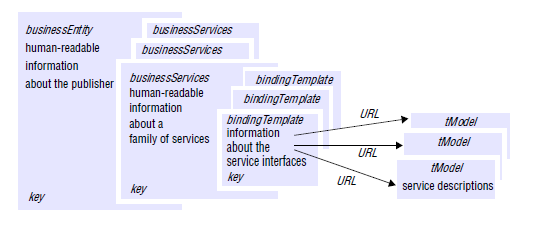
\includegraphics {7/directorio} 
 	 	\caption{Directorio de Servicios}
 	 	\label{fig:dic}
  \end{figure}
  
    UDDI proporiona un API para la ubicaci\'on del servicio:
 		\begin{itemize} 
 			\item 	$get \,xxx$ \: $ get-businessDetail,\: get-ServiceDetail ... $ para la obtenci\'on de un registro en particular.
 			\item  $find\, xxx$ \: $find-business, \: find-Service ... $ usado para la b\'usqueda del servicio en el UDDI.
 		\end{itemize}  	
 		El servidor posee un URI para identificar el API del UDDI.
  
 
  \subsection{Seguridad XML } 
        \index{seguridad XML}
   
  	 Seguridad XML es un conjunto de diseños de la W3C (\WC) para registro, manejo de claves y encriptación. Se relaciona con el servicio web  en el documento \textbf{SOAP} donde se describe  la integridad, confidencialidad y autenticación del mensaje.  En el documento \textbf{SOAP} se definen las etiquetas que indican cuales secciones del documento estan encriptadas o seguras: el documento SOA puede  encriptarse en su totalidad  o parte de ello y puede protegerse el acceso  al documento o parte de ello.
  	 
  	La seguridad del servicio web describe tres mecanismos principales:
  	
  	\begin{itemize}
  		\item Cómo firmar mensajes SOAP para asegurar la integridad. 
  		\item 	Cómo encriptar mensajes SOAP para asegurar la confidencialidad.
  		\item 	Cómo adjuntar tokens de seguridad para determinar la identidad del remitente.
  	 
  	\end{itemize}
  	 
  	 La especificación de la W3C (\WC)  permite una variedad de formatos de firma del documento, algoritmos de cifrado y múltiples dominios de confianza, y está abierta a varios modelos de algoritmos de token de seguridad, como:
  	 \begin{itemize}
  	 	\item certificados X.509
  	 	\item tickets de Kerberos,
  	 	\item ID de usuario/credenciales de contraseña,
  	 	\item Aitenticaci\'on SAML (SAML, Security Assertion Markup Language), y
  	 	\item tokens personalizados.
  	 \end{itemize}
  	 
  	Entre los requerimientos para la especificaci\'on del algoritmo para la seguridad del servicio web:
	\begin{itemize} 
		\item Se debe especificar un algoritmo adecuado para la implementación de la seguridad XML.
		\item El algoritmo usado para encriptación y autenticación de un documento debe ser seleccionado de un conjunto y los nombres de los algoritmos deben ser referenciados dentro del documento XML.
		\item Los documentos XML seguros se firman y/o se encriptan mucho antes de cualquier consideración sobre quién los accederá. 
 			\item El estándar especifica un conjunto de algoritmos que se proporcionarán en cualquier implementación de seguridad XML: Al menos un algoritmo de cifrado y uno de firma.
			\item Los algoritmos utilizados deben se seleccionados de ese conjunto y los nombres de los algoritmos en uso se deben referenciar dentro del documento XML.
			\item La seguridad XML define los nombres de los elementos que se pueden usar para especificar el URI del algoritmo en uso para la firma o el cifrado.
		\end{itemize}


 \subsection{Coordinación}
         \index{coordinación de servicios web}
 
 	  La infraestructura SOAP admite interacciones  de solicitud-respuesta entre clientes y servicios web.  Las aplicaciones  generan solicitudes que deben realizarse en un orden particular. 
 	 Ejemplo, al reservar un vuelo, la información de precio y disponibilidad se recopila antes de realizar las reservas. 
 
		 Cuando un usuario interactúa con páginas web en un navegador, para reservar un vuelo o hacer una oferta en una subasta, la interfaz proporcionada por el navegador controla la secuencia en el que se realizan las operaciones.
		 En un servicio web que realiza reservas, el servicio web debe trabajar a partir de una descripción de la forma apropiada de proceder cuando se interactúa con otros servicios para, por ejemplo, alquiler de coches y reservas de hotel como así como reservas de vuelos
 
 
 	El prop\'osito de la doordinación de servicios web:
	\begin{itemize} 
		\item para generar esquemas de código para un nuevo servicio que quiera participar;
		\item como base para generar mensajes de prueba para un nuevo servicio;
		\item promover un entendimiento común de la colaboración entre servicios;
		\item analizar la colaboración, por ejemplo, para identificar posibles situaciones de punto muerto
	\end{itemize}

El est\'andar W3C (\WC) establece los siguientes aspectos relacionados con la coordinación de servicios web:
\begin{itemize} 
	\item composición jerárquica y recursiva de coreografías;
	\item capacidad de agregar nuevas instancias de un servicio existente y nuevos servicios;
	\item caminos concurrentes, caminos alternativos y la capacidad de repetir una sección de un coreografía;
	\item tiempos de espera variables, por ejemplo, diferentes períodos para mantener reservas;
	\item excepciones, por ejemplo, para tratar con mensajes que llegan fuera de secuencia y de usuario 	acciones tales como cancelaciones;
 
	\item interacciones asíncronas (devoluciones de llamada);
	\item paso por referencia, por ejemplo, para permitir que una empresa de alquiler de coches consulte a un banco para una verificación de crédito en nombre de un usuario;
	\item  marcado \textit{(timestamp)} de las transacciones  que tienen lugar, por ejemplo, para permitir la recuperación;
	\item la capacidad de incluir documentación legible por humanos.
\end{itemize}
%%%%%%%%%%%%%%%%%%%%%%%%%%%%%%%%%%%%%%%%%%%%%%%%%%%%%%%%%%%%%%%%%%%%%%%%%%%%%%%%%%%%%%%%%%%%%%%%%%%%%%

  \section{REST}
           \index{REST}
  
  	\paragraph{REST: Representational State Transfer}
   La transferencia de estado representacional (Rest, representational state transfer)  es un estilo de arquitectura de software para sistemas hipermedia distribuidos como la World Wide Web. El término se originó en el año 2000, en una tesis doctoral sobre la web escrita por Roy Fielding, uno de los principales autores de la especificación del protocolo HTTP y ha pasado a ser ampliamente utilizado por la comunidad de desarrollo de software. 
		\sidecite{Fielding2000}, \sidecite{Erl2013}
		\sidecite{DimitriosGeorgakopoulos2009} 
		\sidecite{Barry2013}
		
	REST establece un conjunto de principios para la arquitectura de servicios:
  	\begin{itemize}			
  		\item Clientes usan URL y HTTP (GET, PUT, DELETE, POST)
  		\item Recursos son representados  en XML
  		\item Enfasis en manipulación de recursos de datos sobre interfaces			
  		
  	\end{itemize}
  	
 	
  	 \paragraph{Agente}
  	   	           \index{agente}
  	 
  	 El agente ess un programa dirigido por eventos que no proporciona una interfaz técnica publicada. Est\'a diseñado para actuar como un intermediario capaz de interceptar mensajes en tiempo de ejecución.   Cuando se intercepta un mensaje, el servicio agente puede realizar un procesamiento activo o pasivo sobre el mensaje.    	 
  	  La lógica de procesamiento del servicio agente se considera activa cuando termina alterando el contenido del mensaje, mientras que la lógica de procesamiento pasivo no lo hace. 
  	 	 
  
  \subsection{Restricciones de servicios REST}
    	           \index{restricciones de REST}
  
  A continuacion se indican las caracteristicas y restricciones que debe cumplir una arquitetura en REST:
  \paragraph{Cliente - Servidor}
  
  
  	\begin{itemize}
  		\item Requiere que un servicio ofrezca una o más capacidades y escuche las solicitudes sobre estas capacidades. 
  		\item Un consumidor  invoca una capacidad enviando el mensaje de solicitud correspondiente, y el servicio rechaza la solicitud o realiza la tarea solicitada antes de enviar un mensaje de respuesta al consumidor.
  		\item Las excepciones que impiden que la tarea continúe son elevadas al consumidor, y el consumidor es responsable de tomar medidas correctivas. 
  	 
		\item La solución debe someterse a un proceso por el cual está sujeta la separación de solicitudes.
		\item  Esto divide la solución en unidades que abordan solicitudes definidas. Estas unidades se componen para formar la solución en tiempo de ejecución.
		\item El conocimiento requerido del consumidor sobre un servicio y el conocimiento requerido del servicio de sus consumidores se limitan a los contenidos del contrato técnico compartido. 
	\end{itemize}
	
	\paragraph{Sin estado}
	     \index{ servidores sin estado}
 
		\begin{itemize}
			\item Cada solicitud  debe contener toda la información necesaria para que el servicio entienda el significado de la solicitud, y todos los datos de estado de la sesión deben devolverse al consumidor del servicio una vez finalizada  cada solicitud 
			\item La lógica del consumidor debe estar diseñada para preservar los datos del estado entre solicitudes y emitir solicitudes que contengan datos de estado.
			\item La solicitud debe contener todos los datos de estado necesarios para que el servicio la procese, y el servicio debe ser capaz de "olvidar" los datos de estado al emitir la respuesta sin comprometer la interacción general.
		 
				\item Las solicitudes intermedias indican que el servicio está \textit{en reposo} y, usa menos recursos de CPU, memoria o red.
				\item El servicio no almacena datos en una instancia de tiempo de ejecución de un consumidor de servicios. Puede almacenar datos de su propio contexto funcional.
			\end{itemize}	
		 
			\begin{figure}%
			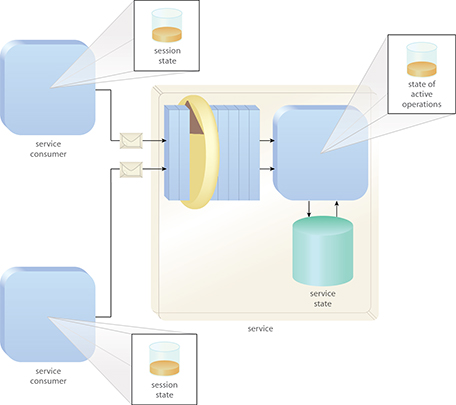
\includegraphics {7/Sin-estado.png} 
				\caption{Servidres sin estado}
				\label{fig:rest-sin-estado}
			\end{figure}
				
			 
	\paragraph{Cache}
	     \index{cache}

	\begin{itemize}
		\item Los mensajes de respuesta del servicio a sus consumidores se etiquetan   como  almacenados o no en caché. 
		\item As\'i, el servicio, el consumidor o uno de los componentes del middleware  pueden almacenar en caché la respuesta para su reutilización en solicitudes posteriores.
		\item Los servicios estan diseñados para producir metadatos para control de caché y devolverlos en mensajes de respuesta. 
		\item Un repositorio de caché intermediario o del lado del consumidor  permite al consumidor reutilizar los datos de respuesta almacenables en caché para los mensajes de solicitud posteriores.  				
		\item Los mensajes de solicitud deben ser comparables para determinar si son equivalentes o no.
		\item Los contratos incluyen declaraciones explícitas sobre la capacidad de almacenamiento en caché de las respuestas, o permitir que los metadatos para control de caché se incluyan en las respuestas.
	\end{itemize}	
 
 \begin{figure}%
 	\includegraphics {7/Cache.png} 
 	\caption{Cache. Tomado de \ER}
 	\label{fig:rest-cache}
 \end{figure}
 
	\paragraph{Interfaz}
	
	     \index{ interfaz en REST}
 
	\begin{itemize}
		\item Los consumidores acceden a las capacidades del servicio a través de métodos, tipos y una sintaxis común del identificador de recursos que están estandarizados en muchos consumidores y servicios.  
		\item Para consumidores y servicios se establece un contrato uniforme con los tipos de métodos genéricos y reutilizables, y la sintaxis del identificador de recursos.
		\item El procesamiento de mensajes del consumidor está diseñado para estar estrechamente unida al contrato uniforme.	
 
		\item El procesamiento de mensajes del consumidor está diseñado para ser desacoplada o poco unida a las capacidades y recursos específicos del servicio.	
		
		\item Los recursos pueden proporcionar enlaces a otros recursos que el consumidor del servicio puede "descubrir" y, opcionalmente, acceder dinámicamente en tiempo de ejecución.
		
		\item Los consumidores pueden "aprender" dinámicamente nuevos tipos de medios para procesar formatos de recursos previamente desconocidos.			
	\end{itemize}

\paragraph{Sistema de capas}

     \index{ sistemas de capas}
 
	\begin{itemize}
		\item Las capas pueden estar compuestas por consumidores y servicios con contratos publicados o componentes de middleware basados en eventos (intermediarios) que establecen capas de procesamiento entre los consumidores y los servicios. 
		\item Los consumidores están diseñados para invocar servicios sin el conocimiento de qué otros servicios también pueden invocarlos.
 
			\item Los intermediarios se agregan para realizar el procesamiento del mensaje en tiempo de ejecución sin conocimiento de cómo esos mensajes pueden procesarse más allá de la siguiente capa de procesamiento.
			\item La arquitectura de la solución está diseñada para permitir que se agreguen nuevas capas de middleware o eliminar capas antiguas de middleware sin cambiar el contrato técnico
			\item Los mensajes de solicitud/respuesta no deben revelar de qué capa proviene el mensaje a sus destinatarios.			
		\end{itemize}

  \paragraph{Código-Por-Demanda}
       \index{código por demanda}
 
	\begin{itemize}
		\item  Las arquitecturas de consumo de servicios incluyen un entorno de ejecución de la lógica proporcionada por un servicio. Esta lógica diferida se puede usar para extender la funcionalidad del consumidor o para especializarlo temporalmente.
		\item Los consumidores de servicios están diseñados para procesar la lógica descargada por los servicios en tiempo de ejecución.
		
		\item Los servicios toman decisiones explícitas sobre si ejecutarán la lógica ellos mismos o diferirán la ejecución de esa lógica a sus consumidores.		
		
	\end{itemize}
	
		\subsection{Metas de un servcios REST}
		       \index{metas de REST}
		       
		Las metas de un servicio REST esta relacionada con lo siguiente:
	\begin{description}
		\item[Rendimiento] La latencia de la red, el ancho de banda de la red limitado,  y las redes no confiables pueden afectar el rendimiento al perder, reordenar o retrasar paquetes o mensajes y exigir que se vuelvan a intentar o reenviar
		
		\item[Escalabilidad]   La necesidad de que una arquitectura admita instancias o interacciones simultáneas. 
		Se identifican cuatro enfoques:
			 \begin{itemize}
				\item escalar, aumentar la capacidad de los servicios, los consumidores y los dispositivos de red
				\item escalamiento, distribución de carga entre servicios y programas
				\item suavizar,  igualar el número de interacciones durante los períodos pico y no pico para optimizar la infraestructura
				\item desacoplamiento del consumo de recursos finitos como la memoria de los consumidores concurrentes	  			
			\end{itemize}
			
		\item[Sencillez]  El objetivo de diseño sencillo se basa en la 	aplicación adecuada de la separación de solicitudes.
			
		  La sencillez es un foco para REST porque tiene un impacto en cómo los servicios se definen, descubren y finalmente se usan (o reutilizan) y además determina la facilidad con la que se pueden desarrollar los servicios de manera independiente.  			
		  La principal contribución de REST a la sencillez es la restricción de contrato uniforme  			
 
		\item[Modificabilidad] La facilidad para hacer cambios en una arquitectura.
		Se divide en las siguientes capacidades:
		\begin{itemize}
			\item 	evolución: refactorizar y volver a implementar componente del servicio, consumidor o middleware, sin afectar otras partes. 
			\item extensibilidad: agregar funcionalidad a la arquitectura (incluso mientras se ejecutan las soluciones).   
			\item personalización: modificar temporalmente partes de una solución para realizar tipos de tareas especiales.
			\item configurabilidad: modificar permanentemente partes de una arquitectura.
			\item reutilización:  agregar nuevas soluciones a una arquitectura que reutilice servicios existentes, middleware, sin modificaciones.			
		\end{itemize}
		
		\item[Visibilidad]  Es la capacidad de as partes de una arquitectura para monitorear y regular la interacción entre otras partes de la misma arquitectura. 
		Se traduce en el establecimiento de servicio agente basados en middleware que realizan un seguimiento de los mensajes transmitidos entre los servicios y los consumidores.
		El enfoque de estos servicio de agentes  es mejorar el control administrativo sobre la arquitectura y optimizar su desempeño. 			
 
		
		\item[Portabilidad]    La facilidad con la que los servicios y las soluciones pueden trasladarse de una ubicación implementada a otra.
		 Las consideraciones que se deben tener en cuenta incluyen el nivel de estandarización compatible en todos los entornos, la capacidad de mantener tanto los datos como la lógica agrupados, y qué tan portátil puede ser un determinado programa de software.	  			
 
		
		\item[Confiabilidad]    Es el grado en que las soluciones y servicios (y la infraestructura subyacente) son susceptibles de fallar.  La confiabilidad de una arquitectura se puede mejorar al evitar puntos únicos de falla, al utilizar mecanismos de conmutación por error y,  funciones de monitoreo que pueden anticiparse y responder dinámicamente a las condiciones de falla.  			
 		
	\end{description}	       
   
      \subsection{Contratos de servicios no-Rest vs servicios REST:}
             \index{contratos no Rest}
             
       \paragraph{Contratos de servicios no-Rest}
       
      En la figura \ref{fig:rest-contratoNR} se muestra un esquema de como trabaja un contrato de servicio \textbf{SOA} usando como ejemplo un servicio de emisi\'on de facturas::
      	\begin{itemize}  			
      		\item Emite un mensaje \textbf{SOAP} para solicitar datos de factura invocando \textit{getInvoice}, predefinido en la definición \textbf{WSDL} contrato de servicio de Factura.
      		\item Recibe datos solicitado de facturas en un mensaje de respuesta \textbf{SOAP} emitido por  \textit{getInvoice} del servicio de Factura.
      		\item Emite un mensaje \textbf{SOAP} para solicitar datos del cliente invocando la capacidad  \textit{GetCustomer}, predefinido en la definición \textbf{WSDL} del contrato de servicio al cliente.
      		\item Recibe los datos solicitados del cliente en un mensaje de respuesta SOAP emitido por la capacidad del servicio \textit{GetCustomer} del servicio al cliente.
      		\item Emite un mensaje \textbf{SOAP} solicitando que se agregue la dirección del cliente a la cola de impresión invocando la capacidad del servicio de impresión del servicio de impresora, como está predefinido en la definición WSDL del contrato de servicio de la impresora.
      		\item Recibe un mensaje de respuesta \textbf{SOAP} que indica que la acción fue exitosa (o no).	
      	\end{itemize}
      	
      	 \begin{figure}%
      		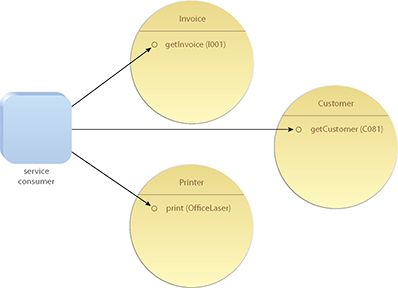
\includegraphics {7/contratoNR.png} 
      		\caption{Contrato SOAP. Tomado de \ER}
      		\label{fig:rest-contratoNR}
      	\end{figure}
       
     
   	En el listado \ref{contrato-soap} es un  ejemplo de un mensaje SOAP simple que es enviado a un contrato de servicio basado en WSDL para solicitar una factura en función de su ID:
   	 
     
  \begin{lstlisting}[label=contrato-soap, label= Solicitud en contrato de servicio SOAP]
	<soap:Envelope>
		<soap:Header>
			<wsa:To>
				 http://invoice/
			</wsa:To>
		</soap:Header>
		<soap:Body>
			<getInvoice>
				<invoice-id>
				      I123
				</invoice-id>
			</getInvoice>
		</soap:Body>
	</soap:Envelope>
  \end{lstlisting}
   
   
   	El ejemplo de  mensaje de respuesta devuelto por el servicio web, en el listado \ref{contrato-soap-resp},  proporciona un mensaje de respuesta en SOAP que contiene el contenido de la factura.
  
   
   
   \begin{lstlisting}[label=contrato-soap-resp, label= Respuesta en contrato de servicio SOAP]
   	<soap:Envelope>
  	 	<soap:body>   	 
  		 	<getInvoiceResponse>
  			 	<invoice> 
  			 		... invoice content...
   				</invoice>
   			</getInvoiceResponse>
   		</soap:body>
   	</soap:Envelope>
   \end{lstlisting}
   
  	\paragraph{Contratos de servicios Rest:}
  	\index{contratos Rest}
    En la figura \ref{fig:rest-contrato} se detallan las   acciones relacionadas con el proceso de solicitud-respuesta del servicio de emisi\'on de facturas usando un contrato REST:
    
    	\begin{itemize}  			
    		\item Emite una solicitud de datos de factura accediendo al servicio de Factura, utilizando un identificador de recursos y procesado mediante el método \textbf{HTTP GET}.
    		\item Recibe los datos de factura solicitados en un mensaje de respuesta \textbf{HTTP} emitido por el servicio Factura.
    		
    		\item Emite una solicitud de datos de clientes accediendo al servicio de atención al cliente, utilizando un identificador de recursos y procesado mediante el método \textbf{HTTP GET}.
    		\item Recibe los datos solicitados del cliente en un mensaje de respuesta \textbf{HTTP} emitido por el servicio al cliente.
    		\item Emite una solicitud para que la dirección del cliente se agregue a la cola de impresión, accediendo al servicio de la impresora utilizando un identificador de recursos y procesado a través del método HTTP POST.
    		\item Recibe una respuesta \textbf{HTTP} indicando que la acción fue exitosa (o no).	
    	\end{itemize}
    
    
    \begin{figure}%
    	\includegraphics {7/contratoR.png} 
    	\caption{Contrato REST. Tomado de \ER}
    	\label{fig:rest-contrato}
    \end{figure}
     
   
    El intercambio  con un servicio REST se basa en el uso de métodos HTTP, ejemplo en el listado \ref{contrato-rest-sol}: 
    	
    	 \begin{lstlisting}[label=contrato-rest-sol, caption=Solicitud en contrato de servicio REST]
    	 	GET http://invoice/invoice/I123 HTTP/1.1
    	 	Accept:application/vnd.com.example.invoice+xml
    	\end{lstlisting}
    	
     El mensaje HTTP de respuesta, listado \ref{contrato-rest-res} que se devuelve al consumidor contiene un código de éxito o falla, el enunciado del encabezado del tipo de medio y el mismo fragmento XML que el mensaje de respuesta del servicio web. 
    
      	 \begin{lstlisting}[label=contrato-rest-res, caption=Respuesta en contrato de servicio REST]
      	 Content-Type:application/vnd.com.example.invoice+xml
	      	 <Invoice>
	      	  	...invoice content ...
	      	 </Invoice>	  	
      	\end{lstlisting}
      	
\section{Caso de Estudio: Monolitos vs Microservicios}

\index{caso de estudio!microservicios} 
\index{caso de estudio!monolitos} 

\subsubsection{Monolitos}

Las aplicaciones monolíticas \sidecite{Richardson2016} \sidecite{Erl2007} consisten en un solo proceso que abarca una sola capa de aplicación, soportando las reglas de negocio, la manipulación de los datos y en ocasiones la interfaz de usuario. Los datos pueden ser almacenados físicamente en una ubicación remota, pero la lógica para su acceso y procesamiento es parte de la  aplicación.

Como se observa en la figura \ref{fig:monolito}, en el núcleo de una aplicación monolítica está la lógica de negocio, que definen los servicios que ofrece el sistema. Alrededor del núcleo están los adaptadores que se conectan con servicios externos, que incluyen componentes de acceso a base de datos, de mensajería web y que exponen la interfaz de programación de la aplicación,  API.

  \begin{figure}%
	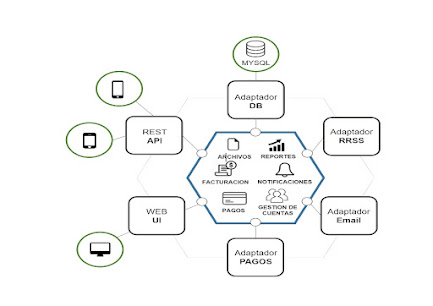
\includegraphics {7/Monolito} 
	\caption{Monolito. Tomado de \cite{Salas2017} }
	\label{fig:monolito}
\end{figure}

\paragraph{Ventajas y desventajas de aplicaciones monolíticas.}

Entre las ventajas se destaca:
\begin{itemize}
	\item Pruebas Unitarias: las aplicaciones monolíticas son fáciles de probar, debido a su popularidad en los últimos años, existen variedades de herramientas para realizar las pruebas unitarias, y debido a que estas aplicaciones corren bajo un mismo proceso, con sólo ejecutar el proceso se pueden hacer las pruebas necesarias.
	\item 	Implementación:  son fáciles de implementar ya que, por lo general, es necesario copiar un único archivo en un directorio. 
	\item Comunicación: ya que en las aplicaciones monolíticas todo está construido en un solo programa, no hay necesidad de una comunicación complicada a través de la red. 
\end{itemize}
 
Y la desventajas de su uso:

\begin{itemize}
	\item Desarrollo: las aplicaciones exitosas tienen el hábito de crecer con el tiempo, este crecimiento s refleja en el incremento de los requerimientos, el alcance de la aplicación  y en la ampliación del equipo de desarrolladores, así como aumento de la complejidad del código. 
	\item Despliegue continuo: Para realizar cambios en producción, es necesario redesplegar toda la aplicación, independientemente de lo que se necesite modificar, resultando difícil su manejo.
	\item Escalabilidad:  cada uno de lo módulos de un  monolito posee requerimientos de hardware distintos, en consecuencia, la capacidad de escalar de manera independiente se convierte en una tarea compleja. 
	\item Resistencia a fallas: ya que todos los módulos que componen las aplicaciones corren sobre un mismo proceso, una falla en cualquiera de estos módulos, puede hacer fallar el proceso completo. 
	\item Heterogeneidad Tecnológica: los módulos de la aplicación corren bajo un mismo proceso, y estos están escritos en un mismo lenguaje de programación con un framework específico, haciendo costoso adoptar nuevas tecnologías.
\end{itemize}

\subsubsection{Microservicios}

El estilo arquitectónico de microservicio \sidecite{Richardson2016} \sidecite{Erl2007} se enfoca en desarrollar una sola aplicación como un conjunto de pequeños servicios, cada uno ejecutándose en su propio proceso y comunicándose con mecanismos ligeros. Estos servicios se basan en capacidades de negocios y son desplegados independientemente mediante cualquier mecanismo de despliegue automatizado

En la figura \ref{fig:microservicio} se observa el esquema de la aplicación presentada en la figura \ref{fig:monolito}, adoptando  un enfoque orientado a microservicios, donde se puede ver que cada módulo de la aplicación monolítica ahora se ha convertido en un microservicio independiente, que interactúa con otros.

 \begin{figure}%
	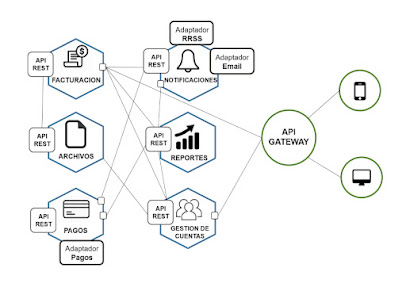
\includegraphics {7/microservicio} 
	\caption{Microservicios. Tomado de \cite{Salas2017} }
	\label{fig:microservicio}
\end{figure}

\paragraph{Ventajas y Desventajas de los Microservicios}
Entre sus ventajas destaca:
\begin{itemize}
	\item Heterogeneidad tecnológica: con un sistema compuesto de múltiples microservicios colaboradores, se puede decidir utilizar diferentes tecnologías dentro de cada uno.
	\item Resistencia: en las aplicaciones basadas en microservicios: si en un microservicio se presenta una falla, esta solo afectará a dicho microservicio, y no a todo el sistema, existen mecanismos de resistencia a fallas para que los otros microservicios continúen trabajando.
	\item Escalabilidad: en microservicios, la escalabilidad se puede aplicar a los microservicios que la necesiten, esto permite que se enfoquen los recursos necesarios a los microservicios que lo requieran.
	\item Fácil despliegue: a diferencia de las aplicaciones monolíticas, que para realizar un cambio en producción se requiere el despliegue de toda la aplicación como una pieza independientemente del tamaño del cambio, en los microservicios, el despliegue es por microservicio; un cambio en un microservicio es independiente de los demás que conformen el sistema.
	\item Reemplazabilidad: En un sistema con microservicios individuales de pequeño tamaño, el costo de reemplazarlos o borrarlos, es menor, que reemplazar alguna funcionalidad de un sistema monolítico.
\end{itemize}

Los  microservicios tienen muchas ventajas, pero no son perfectos; tienen asociados las dificultades que acompañan  a los sistemas distribuidos. 
 Entre sus desventajas:
 
 \begin{itemize}
 	\item Complejidad: por el hecho de que son sistemas distribuidos. Los desarrolladores necesitan elegir e implementar un mecanismo de comunicación entre procesos;  también el  código para manejar fallos parciales.
 	\item Bases de datos: para microservicios se puede manejar varios enfoques para base de datos; es común  el crear una base de datos para cada microservicio, lo cual conlleva a transacciones con múltiples bases de datos. Las transacciones en este tipo de sistema, conllevan a gestionar varias bases de datos pertenecientes a diferentes microservicios.
 	\item Pruebas unitarias:  las pruebas unitarias las cuales son complejas, ya que en este tipo de aplicaciones es necesario acoplar el funcionamiento de los módulos o funciones del sistema que requieran conexiones con otros componentes de la red (bases de datos o microservicios). 
 \end{itemize}

